%\addcontentsline{toc}{chapter}{Development Process}
\chapter{Development Process}

\section{Introduction}
I chose to use the iterative and incremental approach to development.  This is mainly because of how modular my project is.  In theory, I can add more functionality with minor adjustments to the core system, thus making iterative/incremental very suited to my needs.
\\Each part of the system in an incremental strategy can be developed independently and slotted together as they reach completion.
\\Each iteration is a review of the previous which has been reworked and improved upon.
\\For a well functioning system it needs good design, quality programming and a good debugging process.  So, after designing the inital system, writing a simple prototype it is then time for debugging it to get an indication of what the main flaws are.  Once these flaws have been clearly identified a new design has to be drawn up to correct these issues.  After writing the new version following the revised design the cycle continues in the same manner, design, write then debug.


\section{Modifications}
No real modifications were made to this development process as it works for individuals and for teams without alteration.

\section{Version Control}
This is majorly useful in any project which involves managing code or documents digitally.  It is even usefull as a backup tool, to be safe from accidental deletions, hard drive failure or any number of other unfortunate occurances (for instance a fire destroying your computer) as you can just re-download the files.
\\There are other features that version control systems offer that are of more use in this type of project.  Branching and merging are two of the most used features.  These enable the user to make a branch within the project in which they can work on a specific feature independantly of the main project.  You may make multiple branches at the same time and work on different things all independant of each other.  If you imagine a tree, where the trunk contains the current working state of a project, then if you want to change something or create something new you make a branch which shoots off from the tree but contains all the information that is in the trunk.  You can then work on it independantly from the trunk, even if you or somebody else makes another branch from the trunk, the changes made in your branch will not effect it.  Once these are finished you can merge them back into the main project, this is a very nice feature version control systems offer as it performs most, if not all of this for you, instead of having to manualy try and integrate each line of the branch files back into the main ones.
\\I have chosen to use Git for developing this project due to how powerful the merge feature is as well as a website called github \cite{github} which will host repositories for people.  The website also has nice usage statistics and offer some private repositories to students.  Github repositories are normally open to the general public unless you pay a fee for having non public facing ones.  Being a student enables me to have a small number of these private repositories which let me control when I am ready to release a project to public viewing.
\begin{figure}[h]
\centering
        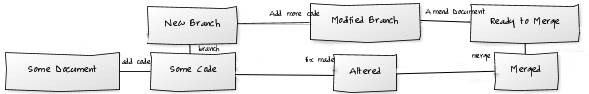
\includegraphics[width=6.0in] {Images/git-branch-merge.png}
        \caption{Branch Merge Diagram}
        \label{Branch Merge Diagram}
\end{figure}
